\documentclass[letter]{ieicej}
\usepackage[dvipdfmx]{graphicx,xcolor}
\usepackage[fleqn]{amsmath}
\usepackage{newtxtext}
\usepackage[varg]{newtxmath}
\usepackage{url}
\typeofletter{研究速報}
\field{}
\jtitle{LLMエージェントの差分要約における保持表現と発動時機の比較}
\etitle{Comparing Retained Representations and Trigger Timing for Delta Summaries in LLM Agents}
\authorlist{\authorentry{著者未設定}{Author details pending}{}{}\MembershipNumber{}}
\jalcdoi{???????????}
\begin{document}
\maketitle
\begin{abstract}
LLMエージェントの差分要約と再提示量による発動を比較する．既知1課題で閾値型差分要約は成功を保ち費用を0.84％減らしたが，再提示量型は失敗した．局所入力縮小と全体成果の分離評価が必要である．
\end{abstract}
\begin{keyword}
LLMエージェント，文脈圧縮，差分要約，再提示量，費用評価
\end{keyword}
\begin{eabstract}
We compare delta-summary representations and trigger timing. On one known AppWorld task, threshold-triggered delta summarization retained success with 0.84\% fewer logical tokens than recursive summarization, while an exposure-based trigger failed. This diagnostic distinguishes local input compression from task success and whole-job cost; generalization remains untested.
\end{eabstract}
\begin{ekeyword}
LLM agents, context compression, delta summarization, exposure, cost evaluation
\end{ekeyword}

\section{まえがき}
大規模言語モデル（LLM）によるエージェントは，推論と行動を繰り返し\cite{yao2023react}，生成したコードで外部環境を操作する\cite{wang2024codeact}．行動と観測の履歴は後続の判断に必要だが，繰り返し入力されるため，長い課題では累積トークン数が増大する．要約により入力を短縮できても，要約自体の推論費用と情報欠落による再試行が生じ得る．したがって，最終的な課題達成を保ちながら，制御処理を含む仕事全体の費用を減らす必要がある．

プロンプト圧縮\cite{jiang2024longllmlingua}，エージェントの観測・履歴圧縮方針の最適化\cite{kang2026acon}，キャッシュを考慮した保持・削除\cite{xu2026tokenpilot}は既に研究されている．本研究は要約そのものではなく，\emph{新たに蓄積した履歴をいつ有料で要約するか}を対象とする．入力長の閾値だけでは，短い履歴が何度も提示された場合と，長い履歴が一度提示された場合を区別できない．そこで，対象履歴の除去前後の入力計数差を累積し，直前の有料要約費用と比較する発動規則を実装する．

本稿の寄与は，既存要約を保持する差分表現と上記の発動規則をハーネスに組み込み，通常の再帰要約との比較に加えて，表現を固定した時点比較を設けた点にある．評価では局所的な入力縮小，要約の実配信，最終成功，全呼出し費用を分離する．少数の既知課題による開発実験として，機構の到達点と適用上の制約を明らかにする．

\section{再提示量を用いる差分要約制御}
\subsection{ハーネスと保持表現}
図\ref{fig:architecture}に構成を示す．actorは課題を進めるLLM呼出し，focusは履歴要約専用のLLM呼出しである．ハーネスは完全な履歴を保存し，actorにはシステム指示，課題，採用済み要約，要約後の履歴から成る表示用入力を渡す．直近2ターンは要約対象から除き，前回の要約機会以後に3ターン以上完了した場合を次の機会の候補とする．

\begin{figure*}[t]
\centering
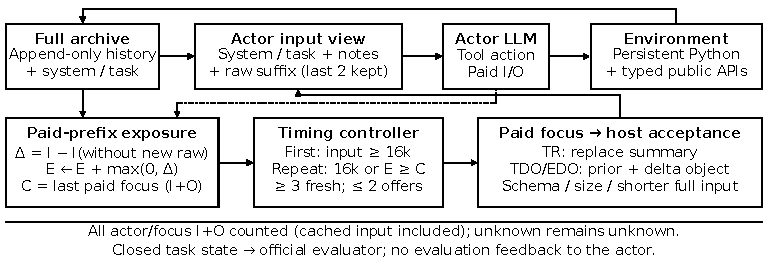
\includegraphics[width=130mm]{figures/architecture.pdf}
\caption{要約の時機と保持表現を分離したハーネス構成．}
\ecaption{Harness separating checkpoint timing from retained representation.}
\label{fig:architecture}
\end{figure*}

比較する方式を表\ref{tab:policies}に示す．TRは現在の入力長を閾値として，旧要約と対象履歴から要約を作り直す通常方式である．TDOは同じ閾値で新規履歴だけの差分を生成させ，host側で旧要約と結合する．EDOはTDOと同じ差分表現を用い，反復時の発動だけを後述の規則へ変更する．初回は全方式で同じ16,384入力トークンの閾値と同じ要約処理を用いる．差分表現は初回の要約が採用済みの第2機会だけに適用する．時機の規則は初回が不採用でも適用される．

\begin{table}[t]
\caption{最終診断に用いる3方式．}
\ecaption{Three policies in the final diagnostic.}
\label{tab:policies}
\centering
\begin{tabular}{lll}
\hline
方式 & 反復時の発動 & 第2要約の表現\\ \hline
TR & 入力長閾値 & 再帰的な置換\\
TDO & 入力長閾値 & 旧要約＋差分object\\
EDO & $E\ge C$ & 旧要約＋差分object\\ \hline
\end{tabular}
\end{table}

差分には単一のJSON objectを明示して要求する．前要約はhostが保持し，新規差分を追加するため，LLMに前要約の再生成を要求しない．結合結果には8,192文字，4つのfieldそれぞれに合計32項目，1項目2,048文字の上限を適用する．構造検査と入力縮小の検査を通過した結果だけをactorに配信する．この検査は構文と長さを扱うものであり，旧要約の正確さや必要情報の保持を保証しない．不採用の有料要約も費用に含める．

\subsection{発動規則}
呼出し$i$の実入力のnative tokenizerによる長さを$W_i$とする．同じシステム指示，課題，tools，予算状態，旧要約，直近履歴を保ち，直前の採用位置以後の新たな要約対象履歴だけを除いた計数専用入力の長さを$U_i$とする．対象履歴の再提示量を
\begin{equation}
 e_i=\max(0,W_i-U_i),\qquad
 E_t=\sum_{i\in\mathcal{A}_t} e_i
 \label{eq:exposure}
\end{equation}
と定める．$\mathcal{A}_t$は直前の費用確定済みfocus以後に完了し，実使用量が確定したactor呼出しの集合である．計数専用入力をactorに送って回答を生成することはない．差分計数による入力帰属自体は先行研究\cite{singh2026tca}にある．ここでは対象を新規の要約可能履歴に限定し，複数回の提示にわたり累積して発動へ用いる．

直前の費用確定済みfocusの実入力と実出力の和を$C_t$とし，EDOは他の適格条件を満たす境界で$E_t\ge C_t$なら次のfocusを提案する．反復時には入力長16,384を併課しない．既に支払った要約費を，次の要約を検討する尺度に用いる経験則である．focusの費用が確定すると，採否にかかわらず$C$を更新し$E$を0へ戻す．未送信なら更新せず，実使用量が不明になった場合はその条件を停止する．1課題当たり最大2回の要約機会には，不採用・未送信も含める．

提案規則は，過去の再提示量が大きい履歴を要約の候補とするが，過去の費用を回収できるわけではない．共通の履歴以後に，方式$p$が支払うfocus費用を$F_p$，actor入力を$I_p$，actor出力を$O_p$とすれば，2方式の全体費用差は
\begin{equation}
 T_A-T_B=(F_A-F_B)-(I_B-I_A)+(O_A-O_B)
 \label{eq:cost}
\end{equation}
である．過去の$E$は右辺に削減額として加算できない．例えば，新たなfocus費用を$F$，その後1回だけのactor入力削減を$s$とすると，同じ出力長・成功でも$0<s<F$なら総費用は増える．これは未測定の仮想例であり，$E\ge C$による償却保証を主張するものではない．

\section{実験方法}
\subsection{課題・実装・評価指標}
AppWorld\cite{trivedi2024appworld}の既知4課題を用いた．課題は写真操作，精算，返金，CSV処理に対応する開発用の固定集合であり，無作為標本や未見テストではない．実装・条件・集計記録を公開する\footnote{\url{https://github.com/sophiria1225/AI-}}．最終成功は実行後の状態に対する公式評価器の判定とし，actorの完了宣言や要約採用で代用しない．評価結果を実行中のactorへ返さない．

actorとfocusには同一のMiniMax-M3（GGUF，IQ4\_XS）を用い，llama.cpp b11669，文脈長65,536，KV cache q8\_0，並列数1で実行した．model seedは57を基点として役割ごとの呼出し数で増分し，world seedは42，温度はactor 1.0，focus 0.7とした．計算機はApple M3 Ultra，メモリ256 GiBである．各条件を新規の実行として処理し，モデル・課題・予算を途中結果に応じて変更しない．

各条件の上限はactorとfocusを合算して80モデル要求，450,000論理入出力トークン，作業1,800秒である．環境APIは第1課題160要求，他の課題80要求を上限とする．出力上限は通常4,096トークンとし，残予算にも制限される．計数処理の実時間は作業時間に含めるが，生成されていないトークンを費用へ加算しない．費用指標$T$は全actor・focusの実入力と実出力の和であり，cached inputも等重みで計上する．これは金銭費用，推論時間，消費電力とは異なる．

未完了の呼出しで実使用量が得られない場合は，既知小計と不明呼出し数を併記する．入力の計数値や予約出力上限を実使用量として補完しない．失敗した条件を除外せず，両条件の会計が確定している比較だけにトークン差を求める．全条件の集計が不成立であっても，既知小計を確定総費用と混同しない．

\subsection{比較の段階と帰属範囲}
通常方式の予備比較（P123）では，単発要約，別呼出し反復要約，actorと同時の反復要約を既知4課題で各1回評価した．この予備比較だけは反復機会の上限を3とし，実際の採用は最大2回だった．別呼出し反復要約を強い通常対照として残した．次の4課題比較（P140）はTR，差分object指定前のED，指定後のEDOを各1回評価した．EDとEDOはともに再提示量による発動を用い，第二focusへの出力指示が異なる．異なる実験群の結果は併合しない．

最終診断（P141）はP140終了後，変更機構が発動した第4課題を選び，表\ref{tab:policies}の順で各1回実行した．TDO対EDOは差分表現を固定した時点比較，TR対TDOは表現とobject指示を合わせた比較，TR対EDOは方式全体の比較である．時点の比較では，最初に発動判定が分かれた境界までの入力・観測の対応と，同じ境界での実際の送信先の差を別々に検査する．protocol IDのみを正規化した一致と，文字列の厳密一致は区別する．同一seedだけを根拠に軌跡の一致を仮定しない．

この診断は失敗結果を見た後の既知1課題・固定順序の比較である．後続入力や行動も方式に応じて変わり，計算機状態，キャッシュ，実行順序の影響も残る．採用判定の実験とはせず，元の4課題比較や未見課題の確認を置き換えない．

\section{結果と考察}
\subsection{通常対照と4課題比較}
P123では3方式とも4/4成功し，使用量不明は0だった．全課題の費用は単発893,529，別呼出し反復785,656，同時反復836,922トークンであった．別呼出し反復は単発より12.07\%少なく，差は第4課題に集中した．この結果は通常方式の選定根拠であり，提案する発動規則の改善として扱わない．

\begin{table}[t]
\caption{P140の既知4課題の結果．不明は呼出し数．}
\ecaption{Results on four known tasks in P140. Unknown counts calls.}
\label{tab:p140}
\centering
\begin{tabular}{lrrr}
\hline
方式 & 成功 & 既知token小計 & 不明\\ \hline
TR & 4/4 & 785,656 & 0\\
ED & 3/4 & 861,995 & 1\\
EDO & 3/4 & 770,988 & 1\\ \hline
\end{tabular}
\end{table}

P140の結果を表\ref{tab:p140}に示す．最初の3課題の費用は各方式で一致し，その小計は453,068であった．これらでは変更対象の第二差分要約が発動しなかったため，成功を差分機構の効果に帰属できない．第4課題ではTRが成功し332,588トークン，EDは時間切れで失敗し408,927既知トークンと使用量不明1件，EDOも時間切れで失敗し317,920既知トークンと不明1件となった．EDOの小計がTRより少なくても，成功維持と確定総費用の削減は成立しない．

EDOでは第二差分が採用され，採用境界でactor表示用入力は14,027から6,058トークンへ短縮された（図\ref{fig:local}）．しかし，その後の課題達成には至らなかった．構造化した差分を実際に配信できること，局所入力が短くなること，仕事全体が安く成功することは別の性質である．この区別が，最終診断で時点と表現を切り分ける動機となった．

\begin{figure}[t]
\centering
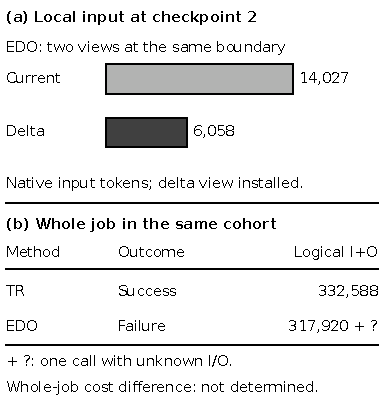
\includegraphics[width=65mm]{figures/task4_local_vs_job.pdf}
\caption{P140第4課題の局所入力と全体結果．$+?$は使用量不明1呼出し．}
\ecaption{Local inputs and whole-job outcomes on task 4 in P140. $+?$ denotes one call with unknown usage.}
\label{fig:local}
\end{figure}

% Actual closed P141, source head 5cab33a2e239f3e6d90e63e32c54ba0764b1c594.
% Original pipeline closed 2026-10-28 03:36 JST; no interim outcome selection.
\subsection{表現を固定した最終診断}
P141の全3条件を評価した結果を表\ref{tab:p141}に示す．TRとTDOは成功し，費用はそれぞれ332,588，329,781トークンであった．TDOはTRより2,807トークン（0.84\%）少なく，内訳はactorの差2,753，要約の差54である．モデル要求は31から30へ減ったが，API要求は76から78へ増えた．第二差分は採用され，費用が確定した7回のactor入力で使用された．この1課題では表現とobject指示を合わせた変更に小さな改善が観測された．

\begin{table}[t]
\caption{P141の既知第4課題の結果（各1回）．}
\ecaption{Final diagnostic on known task 4 in P141, one run per policy.}
\label{tab:p141}
\centering
\begin{tabular}{llrr}
\hline
方式 & 成否 & 既知token小計 & 不明\\ \hline
TR & 成功 & 332,588 & 0\\
TDO & 成功 & 329,781 & 0\\
EDO & 失敗 & 317,920 & 1\\ \hline
\end{tabular}
\end{table}

同じ差分表現を用いるEDOは失敗し，使用量不明が1件残った．TDOとEDOの発動判定は19モデル呼出し後の境界で初めて分かれ，その境界の実際の送信役割も異なり，両送信の費用は確定していた．境界までの履歴は，検証済みprotocol IDを正規化すると一致したが，厳密一致は成立しなかった．TRとTDOの表現変更前も，同じく正規化一致のみ成立した．これらは保存された入力・観測の対応を示す検査であり，隠れた状態や意味の同一性を保証しない．

したがって，表現を同じにしても発動方式の変更後に成功が維持されない例を得た．ただし，最終比較は事後選定した1課題の記述的診断であり，TDOの採用を確認した実験ではない．0.84\%を一般的な改善率とせず，P140の非発動3課題を加えて4課題で確認したとも扱わない．EDOを含む確定費用差は算出できない．


\subsection{研究意義と限界}
本方式はモデルの再学習を要せず，ハーネスで観測できる再提示量と既支出の要約費用から発動を判断する．圧縮方針自体を最適化するACONや，キャッシュ効率を重視するTokenPilotとは，制御入力と評価指標を区別できる．ただし，差分計数，段階的な要約，有料圧縮の費用評価は既存の要素であり，これら単体の新規性や既存法全体への優越性は主張しない．

再提示量の規則は将来の再利用回数や残作業量を含まず，償却を保証しない．今回も再提示量型では成功維持と全仕事削減を確認できなかったが，その原因を単一要因に特定することはできない．旧要約の保持も内容の陳腐化や新規差分の欠落を防ぐ保証ではない．残作業に対する再利用見込みと必要情報の検査は，追加制御費用とともに検討すべき課題である．本稿の課題数・seed・反復数では統計的な非劣性や未見課題への一般化は検証できず，未見12課題の確認実験は実施していない．

\section{むすび}
旧要約を保持する差分表現と，履歴の累積再提示量による発動を実装し，保持表現と時機を切り分けて比較した．既知1課題では閾値型の差分要約が成功を保ち0.84\%の費用減を示した一方，再提示量型は成功を失った．この限定的な結果は，局所圧縮だけでなく，発動後の課題達成と要約費を含む全体費用を評価する必要性を示す．

% Verified official publication metadata; all authors retained.
% Bibliographic source URLs and detailed verification are in references.bib
% and the private claim-source mapping. Only TCA below is a preprint.
\begin{thebibliography}{9}
\bibitem{yao2023react}
S. Yao, J. Zhao, D. Yu, N. Du, I. Shafran, K. Narasimhan, and Y. Cao,
``ReAct: Synergizing reasoning and acting in language models,''
Proc. ICLR, May 2023.

\bibitem{wang2024codeact}
X. Wang, Y. Chen, L. Yuan, Y. Zhang, Y. Li, H. Peng, and H. Ji,
``Executable code actions elicit better LLM agents,''
Proc. ICML, PMLR, vol.235, pp.50208--50232, July 2024.

\bibitem{jiang2024longllmlingua}
H. Jiang, Q. Wu, X. Luo, D. Li, C.-Y. Lin, Y. Yang, and L. Qiu,
``LongLLMLingua: Accelerating and enhancing LLMs in long context scenarios via prompt compression,''
Proc. ACL, vol.1, pp.1658--1677, Aug. 2024.
doi: 10.18653/v1/2024.acl-long.91.

\bibitem{kang2026acon}
M. Kang, W.-N. Chen, D. Han, H. A. Inan, L. Wutschitz, Y. Chen,
R. Sim, and S. Rajmohan,
``ACON: Optimizing context compression for long-horizon LLM agents,''
Proc. ICML, PMLR, vol.306, pp.55321--55375, July 2026.

\bibitem{xu2026tokenpilot}
B. Xu, Z. Xue, D. Chen, C. Fu, C. Wu, C. Huang, C. Jiang, J. Fang,
X. Deng, Y. Chen, Y. Yao, X. Wang, J. Shang, H. Chen, and N. Zhang,
``TokenPilot: Cache-efficient context management for LLM agents,''
Findings of ACL: EMNLP 2026, pp.19034--19049, Oct. 2026.

\bibitem{singh2026tca}
V. K. Singh, P. Priyam, and G. Bhowmick,
``Total cost of agency: Exact attribution of memory injection cost in multi-agent LLM workflows,''
arXiv preprint arXiv:2609.23790v1, Sept. 2026.
\bibitem{trivedi2024appworld}
H. Trivedi, T. Khot, M. Hartmann, R. Manku, V. Dong, E. Li, S. Gupta,
A. Sabharwal, and N. Balasubramanian,
``AppWorld: A controllable world of apps and people for benchmarking interactive coding agents,''
Proc. ACL, vol.1, pp.16022--16076, Aug. 2024.
doi: 10.18653/v1/2024.acl-long.850.

\end{thebibliography}

\end{document}
